\documentclass[a4paper]{article}

%\setlength{\parskip}{0.5\baselineskip}

\usepackage{geometry}
\geometry{left = 2.54 cm, right = 2.54 cm, top = 2.54 cm, bottom = 2.54 cm}

\usepackage{setspace}
\renewcommand{\baselinestretch}{1.0}
\usepackage{indentfirst}
\setlength{\parindent}{2em}

%\usepackage{fontspec}
%\setmainfont{Times New Roman}

\usepackage[]{cprotect}

\usepackage{hyperref}
\hypersetup{
  colorlinks=true,
  linkcolor=blue,
  filecolor=magenta,
  urlcolor=cyan,
}

\usepackage{ulem}
\usepackage{graphicx}
%\usepackage{wrapfig}
\usepackage{enumitem}
\usepackage{xcolor}
\usepackage{subcaption}
\usepackage{float}
\usepackage{amsmath, amssymb, amsthm}
\usepackage{booktabs}

\usepackage{listings} % Required for insertion of code

\lstdefinestyle{lzx}{
    % basicstyle = \small\ttfamily\fontfamily{cmr}\selectfont,
    basicstyle = \ttfamily \footnotesize,
    keywordstyle = \color{purple}\bfseries,
    % commentstyle = \color{green}\itshape,
    commentstyle = \color[RGB]{116, 153, 62}\ttfamily,
    stringstyle = \ttfamily,
    %
    tabsize = 2,
    showspaces = false,
    numberstyle = \ttfamily\color[RGB]{0,96,96},
    showstringspaces = false,
    captionpos = t,
    %
    showlines = true,
    emptylines = *2, % 2 for python, 1 for other language
    numbers = left,
    xleftmargin = 5mm,
    numbersep = 5pt,
    linewidth = \linewidth,
    % backgroundcolor=\color{red},
    frame = single,
    frameround = tttt,
    framexleftmargin = 7mm,
    %
    breaklines = true,
    postbreak = \mbox{\textcolor{red}{\( \hookrightarrow \)}\space},
}

\lstset{
    style = lzx, %
}

%\pagestyle{empty} % Not showing page number

\begin{document}
\renewcommand{\thesection}{\Roman{section}}
\renewcommand{\thesubsection}{\Alph{subsection}}
\renewcommand{\thesubsubsection}{\thesubsection.\arabic{subsubsection}}
\renewcommand{\d}{\: \mathrm{d}}
\newcommand{\e}{\mathrm{e}}

\begin{center}
  \textbf{\Large VE373 Recitation Class}\\[1em]
  \textbf{\large Week 7} \\[1em]
  2022.06.25 \\[1em]
\end{center}

\section*{L11 --- Serial Communication: UART}
  \begin{enumerate}[label = \arabic*.]
    \item \textbf{Serial \& Parallel Communication}
      \begin{figure}[H]
        \centering
        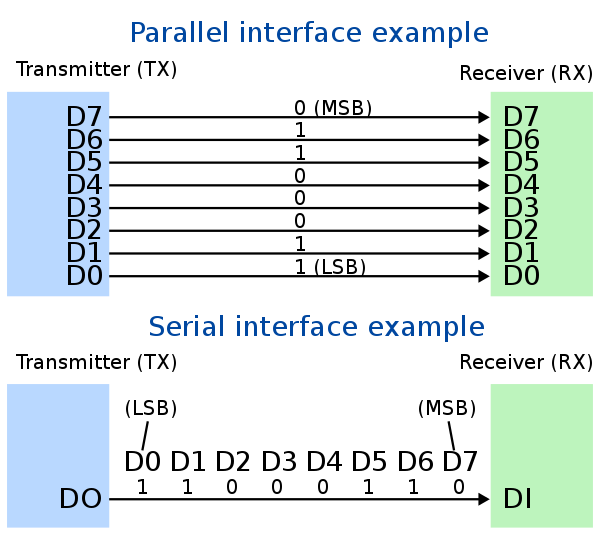
\includegraphics[width=0.4\linewidth]{Serial_parallel_communication.png}
        \label{fig:Serial_parallel_communication.png}
      \end{figure}

      \par Why not parallel communication?
      \begin{itemize}[leftmargin = 1cm]
        \item Parallel I/O uses many signal pins - expensive
        \item Synchronization problem over longer distance
        \item High speed, but many applications do not need high data rate
      \end{itemize}

    \item \textbf{Serial Modules}
      \begin{itemize}[leftmargin = 1cm]
        \item UART (Universal Asynchronous Receiver and Transmitter)
        \item SPI (Synchronous Peripheral Interface)
        \item I2C (Inter-Integrated Circuit)
        \item USB (Universal Serial Bus)
      \end{itemize}

    \item \textbf{Simplex and Duplex Transmission}
      \begin{figure}[H]
        \centering
        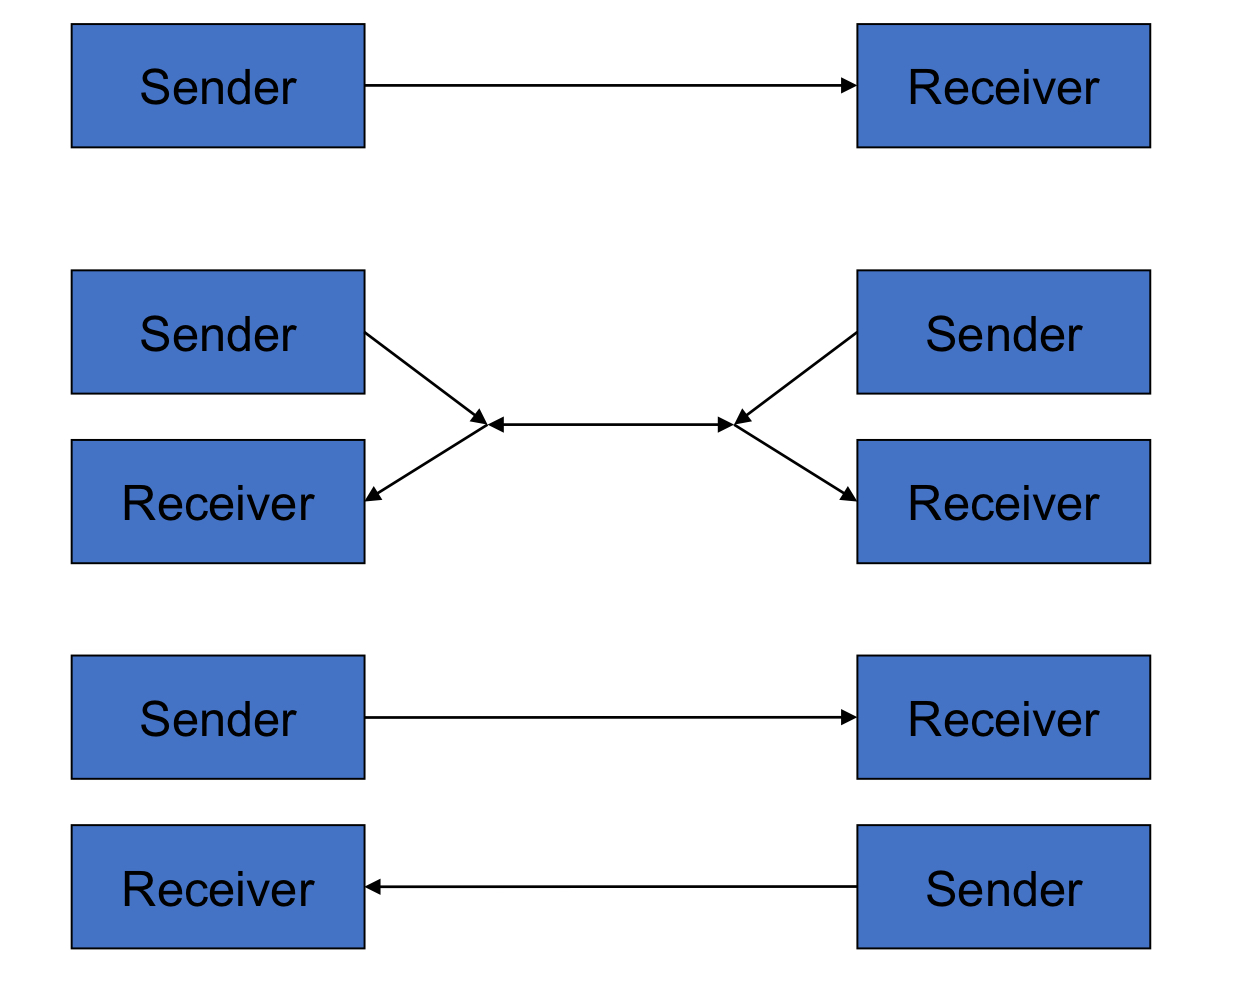
\includegraphics[width=0.4\linewidth]{Simplex_duplex_transmission.jpeg}
        \label{fig:Simplex_duplex_transmission.jpeg}
      \end{figure}

      \begin{itemize}[leftmargin = 1cm]
        \item \textbf{Simplex}: sender can send the data but the sender can't receive the data. It is a unidirectional communication.
        \item \textbf{Half-Duplex}: sender can send the data and also can receive the data one at a time. It is two-way directional communication but one at a time.
        \item \textbf{Full-Duplex}: sender can send the data and also can receive the data simultaneously. It is two-way directional communication simultaneously.
      \end{itemize}

    \item \textbf{Transmission Timing}
      \begin{itemize}[leftmargin = 1cm]
        \item \textbf{Asynchronous}: clock signal not transmitted, receiver and transmitter have there own clocks.
        \item \textbf{Synchronous}: clock signal transmitted.
      \end{itemize}

    \item \textbf{Data Framing}
      \begin{figure}[H]
        \centering
        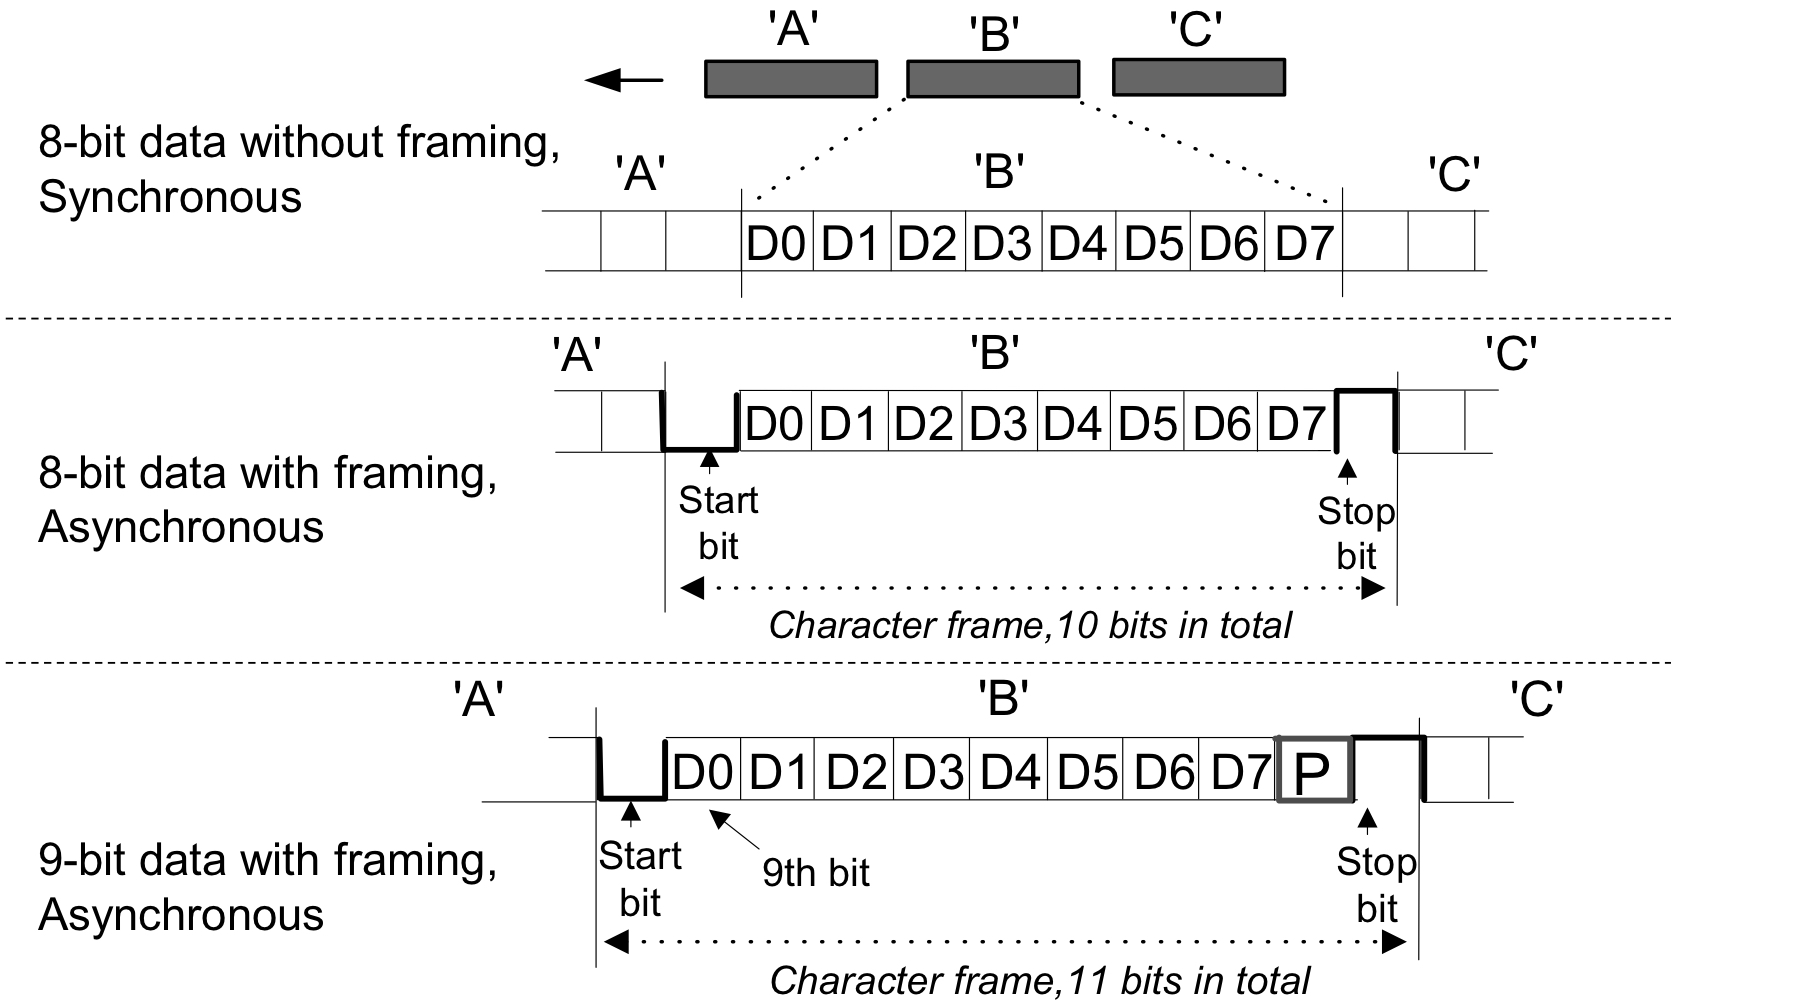
\includegraphics[width=0.8\linewidth]{Data_framing.jpeg}
        \label{fig:Data_framing.jpeg}
      \end{figure}

    \item \textbf{Data Transfer Rate}
      \par Two measurements:
      \begin{itemize}[leftmargin = 1cm]
        \item \textbf{Bps}: bits per second
        \item \textbf{Baud rate}: signaling event per second
      \end{itemize}

      \par One signaling event is possible to transmit multiple bits, i.e., \( \text{Bps} \ge \text{Baud rate} \).

      \begin{figure}[H]
        \centering
        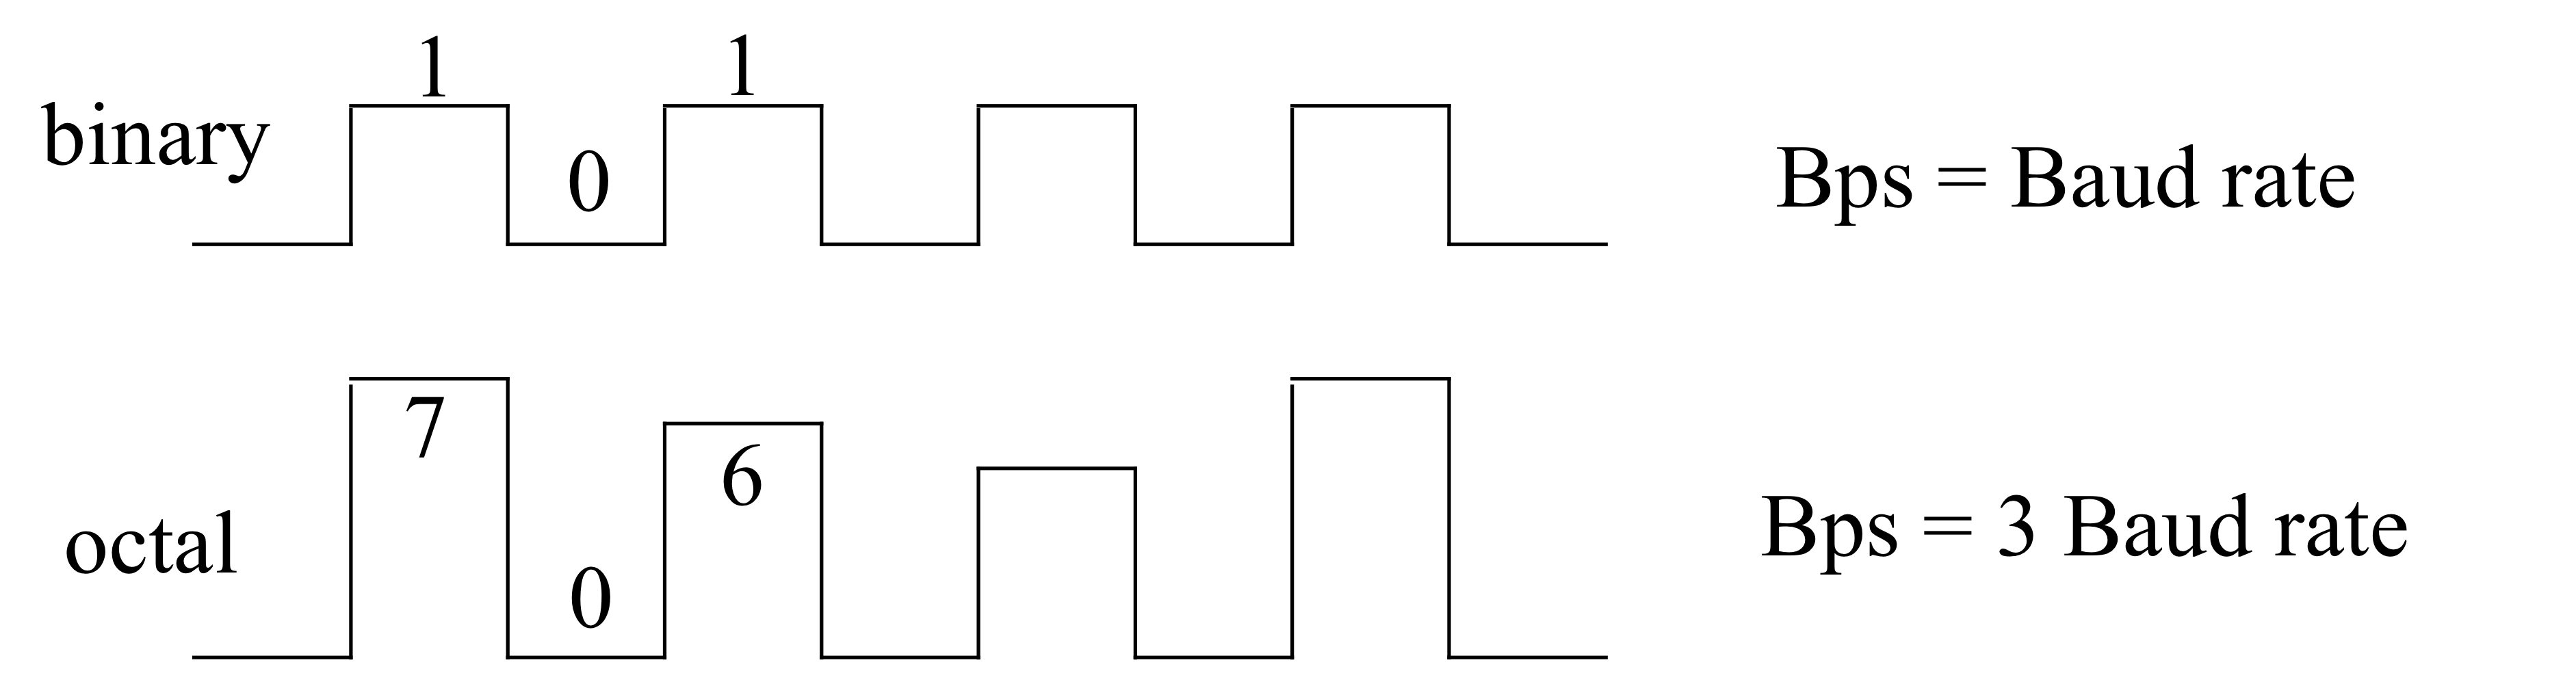
\includegraphics[width=0.6\linewidth]{Baud_and_bit_rate.jpeg}
        \label{fig:Baud_and_bit_rate.jpeg}
      \end{figure}

    \item \textbf{UART in PIC32}
      \begin{itemize}[leftmargin = 1cm]
        \item Full-duplex, 8-bit or 9-bit data transmission
        \item Even, Odd or No Parity options (for 8-bit data)
        \item One or two Stop bits
        \item 8-level deep First-In-First-Out (FIFO) transmit data buffer
        \item 8-level deep FIFO receive data buffer
        \item Up to 6 UART modules
          \begin{itemize}[leftmargin = 1cm]
            \item \verb|UART1A|, \verb|1B|, \verb|2A|, \verb|2B|, \verb|3A|, \verb|3B|
            \item \verb|UARTxB| only available when \verb|UARTxA| is in simple operation mode
          \end{itemize}
        \item Supports multiple communication protocols
          \begin{itemize}[leftmargin = 1cm]
            \item RS-232, RS-485, IrDA, \dots
          \end{itemize}
        \item UART-Related Pins
          \begin{itemize}[leftmargin = 1cm]
            \item \verb|UxTX|, \verb|UxRX|, \verb|UxRTS|, \verb|UxCTS|
          \end{itemize}
        \item UART Control SFRs
          \begin{itemize}[leftmargin = 1cm]
            \item \verb|UARTx| Mode Register (\verb|UxMODE|)
            \item \verb|UARTx| status and control register (\verb|UxSTA|)
            \item \verb|UARTx| Transmit register (\verb|UxTXREG|)
            \item \verb|UARTx| Receive register (\verb|UxRXREG|)
            \item \verb|UARTx| Baud rate generate register (\verb|UxBRG|)
            \item Interrupt registers
              \par For transmitter, receiver, error
          \end{itemize}
      \end{itemize}

    \item \textbf{UART connection pins}
      \begin{figure}[H]
        \centering
        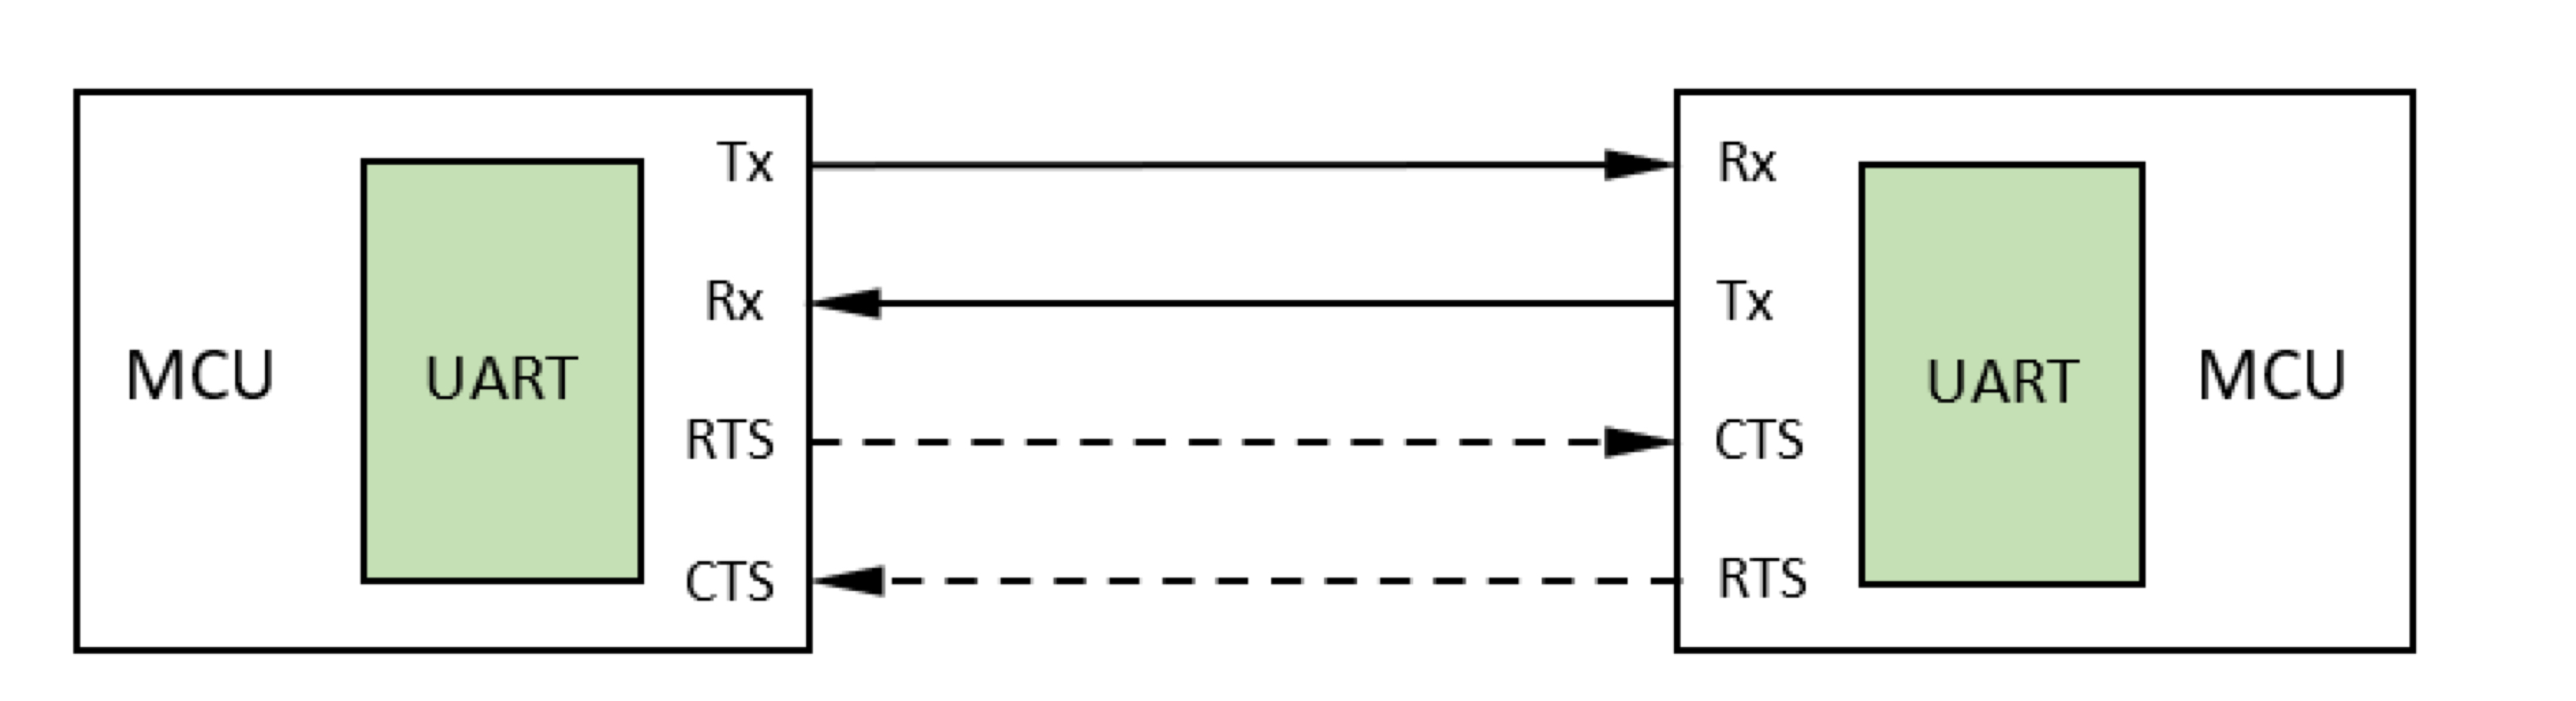
\includegraphics[width=0.6\linewidth]{UART_connection_pins.jpeg}
        \label{fig:UART_connection_pins.jpeg}
      \end{figure}

      \begin{itemize}[leftmargin = 1cm]
        \item \verb|RX|: receiving data, usually an input connected to the TX line of the transmitter
        \item \verb|TX|: transmitting data, usually an output connected to the RX line of the receiver
        \item \verb|RTS| (Request to Send): signal telling transmitter that receiver is ready to receive data. This is usually an output connected to the CTS line of the transmitter
        \item \verb|CTS| (Clear to Send): signal used by a transmitter to identify the situation that is OK to transmit data. This is usually an input connected to the RTS line of the receiver
      \end{itemize}

    \item \textbf{Transmitter block diagram}
      \begin{figure}[H]
        \centering
        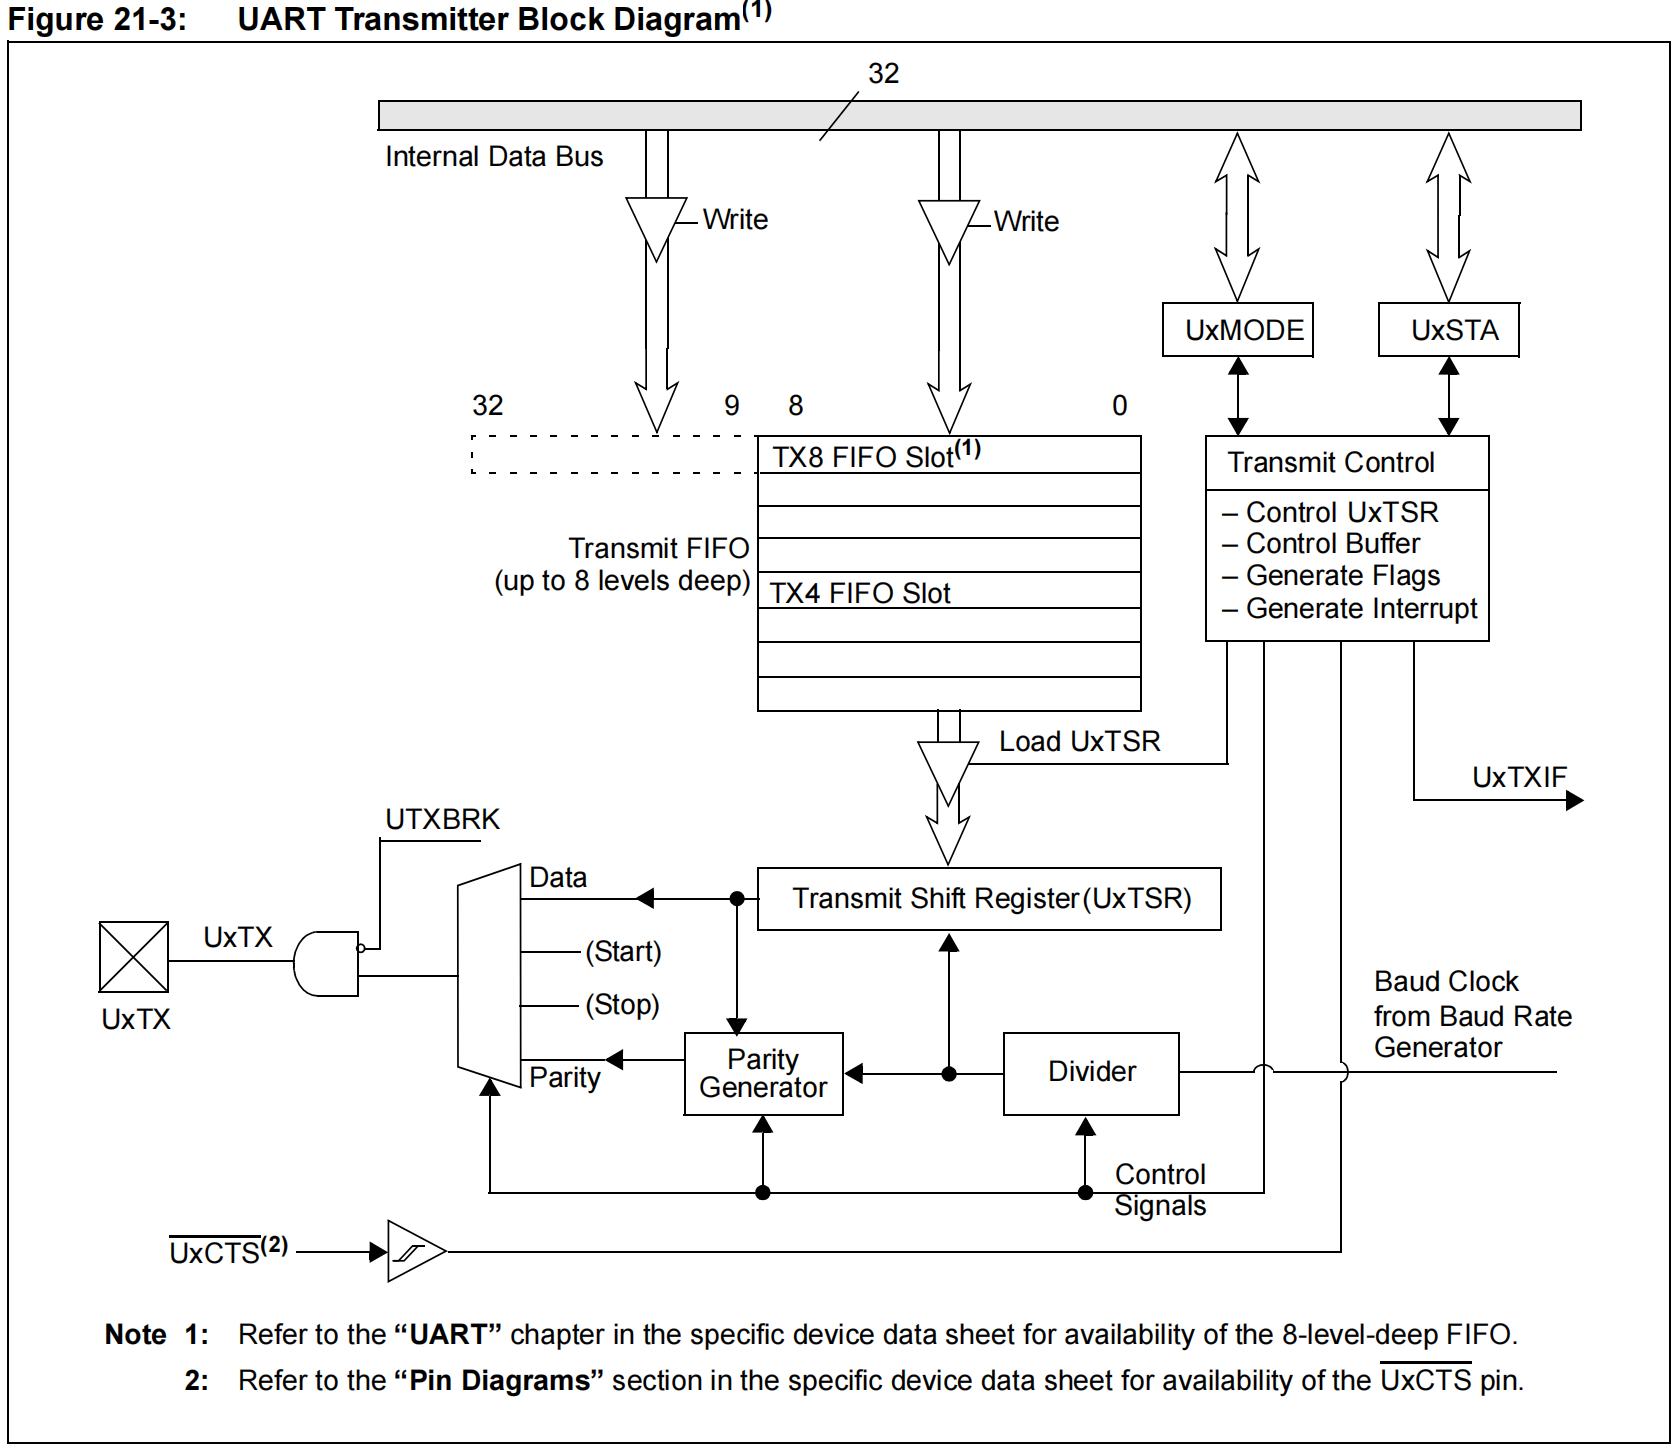
\includegraphics[width=0.8\linewidth]{UART_transmitter_block_diagram.png}
        \label{fig:UART_transmitter_block_diagram.png}
      \end{figure}

    \item \textbf{Baud Rate Generator}
      \par The transmit and receive clock for the UART is generated by the baud rate generator (\verb|UxBRG|)
      \par \verb|UxBRG| specifies the period of a free running 16-bit timer
      \begin{itemize}[leftmargin = 1cm]
        \item \textbf{Standard Speed Mode} (\verb|BRGH = 0|)
          \begin{equation*}
            \begin{aligned}
              \text{Baud Rate} & = \frac{F_{PB} }{16 \cdot (\text{UxBRG} + 1)}   \\
              \text{UxBRG}     & = \frac{F_{PB} }{16 \cdot \text{Baud Rate}} - 1 \\
            \end{aligned}
          \end{equation*}
        \item \textbf{High-Speed Mode} (\verb|BRGH = 1|)
          \begin{equation*}
            \begin{aligned}
              \text{Baud Rate} & = \frac{F_{PB} }{4 \cdot (\text{UxBRG} + 1)}   \\
              \text{UxBRG}     & = \frac{F_{PB} }{4 \cdot \text{Baud Rate}} - 1 \\
            \end{aligned}
          \end{equation*}
      \end{itemize}

    \item \cprotect\textbf{Transmit Buffer (\verb|UxTXREG|)}
      \begin{itemize}[leftmargin = 0.5cm]
        \item 9 bits wide, and up to 8 levels deep.
        \item Together with the Transmit Shift registers (\verb|UxTSR|), the user can have up to a 9-level-deep buffer.
        \item The \verb|UTXBF| status bit (\verb|UxSTA<9>|) is set whenever the buffer is full.
        \item If a user attempts to write to a full buffer, the new data will not be accepted into the FIFO.    \end{itemize}

    \item \textbf{Transmission Interrupt}
      \begin{itemize}[leftmargin = 0.5cm]
        \item \verb|UxTXIF| is generated as soon as the UART module is enabled
        \item \verb|UTXISEL| (\verb|UxSTA<15:14>|) determines when \verb|UxTXIF| flags
        \item \verb|UxTXIF| for status of the \verb|UxTXREG|
        \item \verb|TRMT| bit (\verb|UxSTA<8>|) for status of the UxTSR register
        \item Persistent interrupt: data must be read from, or written to, the \verb|UxRXREG| or \verb|UxTXREG| registers to obtain the number of data to receive/transmit below the level specified by the \verb|URXISEL<1:0>| and \verb|UTXISEL<1:0>| bits.
      \end{itemize}

    \item \textbf{Transmission Setup}
      \begin{enumerate}[label = \arabic*.]
        \item Initialize the UxBRG register for the appropriate baud rate.
        \item Set the number of data and Stop bits, and parity selection by writing to the \verb|PDSEL<1:0>| bits (\verb|UxMODE<2:1>|) and \verb|STSEL| bit (\verb|UxMODE<0>|).
        \item If transmit interrupts are desired
          \begin{enumerate}[label = \arabic*.]
            \item Set \verb|UxTXIE|.
            \item Specify the interrupt priority and subpriority.
            \item Also, select the Transmit Interrupt mode by writing to the \verb|UTXISEL| bits (\verb|UxSTA<15:14>|).
          \end{enumerate}
        \item Enable the transmission by setting the \verb|UTXEN| bit (\verb|UxSTA<10>|), which also sets the UxTXIF bit. The UxTXIF bit should be cleared in the software routine that services the UART transmit interrupt.
        \item Enable the UART module by setting the \verb|ON| bit (\verb|UxMODE<15>|).
        \item Load data to the \verb|UxTXREG| register (starts transmission).
      \end{enumerate}

    \item \textbf{Receiver block diagram}
      \begin{figure}[H]
        \centering
        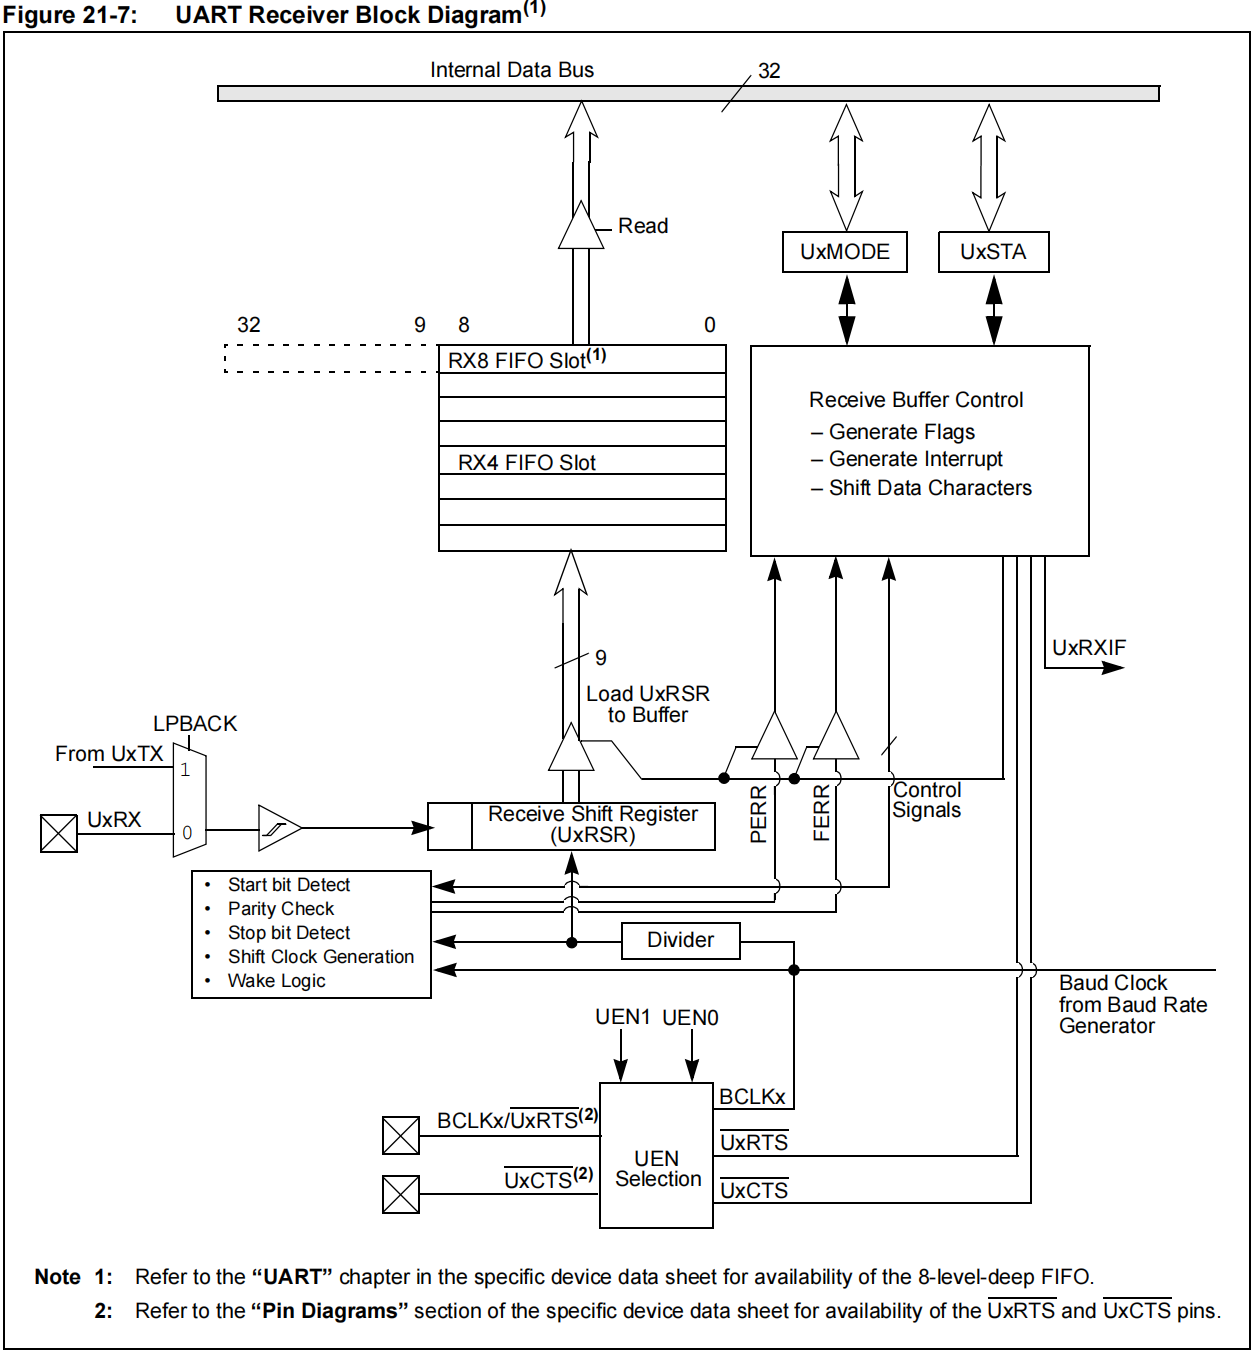
\includegraphics[width=0.8\linewidth]{UART_receiver_block_diagram.png}
        \label{fig:UART_receiver_block_diagram.png}
      \end{figure}

    \item \textbf{Receiver Error Handling (Not covered)}
      \par If the FIFO is full and a new character is fully received into the \verb|UxRSR| register, the overrun error bit, \verb|OERR| (\verb|UxSTA<1>|), is set. The word in \verb|UxRSR| register is not kept, and further transfers to the receive FIFO are inhibited as long as the \verb|OERR| bit is set. The user must clear the \verb|OERR| bit in software to allow further data to be received.

      \par The data in the receive FIFO should be read prior to clearing the \verb|OERR| bit. The FIFO is reset when the \verb|OERR| bit is cleared, which causes all data in the buffer to be lost.
    \item \textbf{Reception Interrupt}
      \begin{itemize}[leftmargin = 0.5cm]
        \item \verb|UxRXIF|, determined by \verb|RXISEL<1:0>| (\verb|UxSTA<7:6>|)
        \item Before clearing the corresponding \verb|UxRXIF| flag bit, the user application must ensure that the interrupt condition specified by the \verb|URXISEL| control bits is no longer true.
        \item \verb|URXDA| (and \verb|UxRXIF|) indicate the status of the \verb|UxRXREG|
        \item \verb|URXDA| (\verb|UxSTA<0>|) indicates whether the receive buffer has data or is empty. Read-only
        \item \verb|RIDLE| (\verb|UxSTA<4>|) shows the status of the \verb|UxRSR| register. Read-only
      \end{itemize}

    \item \textbf{Reception Setup}
      \begin{enumerate}[label = \arabic*.]
        \item Initialize the \verb|UxBRG| register for the appropriate baud rate.
        \item Set the number of data and Stop bits, and parity selection by writing to the \verb|PDSEL<1:0>| (\verb|UxMODE<2:1>|) and \verb|STSEL| (\verb|UxMODE<0>|) bits.
        \item If interrupts are desired
          \begin{enumerate}[label = \arabic*.]
            \item Set the \verb|UxRXIE| bit.
            \item Specify the priority and subpriority for the interrupt.
            \item Also, select the Receive Interrupt mode by writing to the \verb|URXISEL<1:0>| bits (\verb|UxSTA<7:6>|).
          \end{enumerate}
        \item Enable the UART receiver by setting the \verb|URXEN| bit (\verb|UxSTA<12>|).
        \item Enable the UART module by setting the \verb|ON| bit (\verb|UxMODE<15>|).
        \item Receive interrupts are dependent on the \verb|URXISEL<1:0>| bit settings.
          \par If receive interrupts are not enabled, the user can poll the \verb|URXDA| bit (\verb|UxSTA<0>|).
        \item Read data from the receive buffer.
          \begin{itemize}[leftmargin = 0.5cm]
            \item If 9-bit transmission is selected, read a word; otherwise, read a byte.
            \item The \verb|URXDA| bit is set whenever data is available in the buffer.
          \end{itemize}
      \end{enumerate}

  \end{enumerate}

\end{document}